% !TeX program = lualatex
% !BIB program = bibtex
% Auriga theme
% https://github.com/anishathalye/auriga


% Notes:
% - Spelling on slides 47-48

\documentclass[14pt,aspectratio=169]{beamer}
\usepackage{pgfpages}
\usepackage{fancyvrb}
\usepackage{tikz}
\usepackage{pgfplots}

\usepackage[style=authortitle,backend=bibtex]{biblatex}
\addbibresource{../Paper/references.bib}

% \ifnotes
% \setbeamertemplate{note page}[plain]
% \setbeameroption{show notes on second screen=right}
% \fi

\usetheme{auriga}
\usecolortheme{auriga}

\usepackage{hyperref}

\usepackage{tikz}
\usetikzlibrary{positioning}
\usepackage[american]{circuitikz}
\usepackage{tkz-euclide}
\usepackage{listings}

% define some colors for a consistent theme across slides
\definecolor{red}{RGB}{181, 23, 0}
\definecolor{blue}{RGB}{0, 118, 186}
\definecolor{gray}{RGB}{146, 146, 146}

\title{A Comparison of Virtual Analog Modelling Techniques}

\author{Jatin Chowdhury}

\institute[shortinst]{Center for Computer Research in Music and Acoustics (CCRMA)}

\begin{document}

% {
%   % rather than use the frame options [noframenumbering,plain], we make the
%   % color match, so that the indicated page numbers match PDF page numbers
%   \setbeamercolor{page number in head/foot}{fg=background canvas.bg}
%   \begin{frame}
%     \titlepage
%   \end{frame}
% }

% macro to show an image as a full slide
\def\fullslideimg#1{%
\setbeamertemplate{navigation symbols}{}
\begin{frame}<article:0>[plain]
    \begin{tikzpicture}[remember picture,overlay]
        \node[at=(current page.center)] {
            \includegraphics[keepaspectratio,
                             width=\paperwidth,
                             height=\paperheight]{#1}
        };
    \end{tikzpicture}
\end{frame}}

\fullslideimg{Figures/title.jpg}

\begin{frame}{About me...}
    \vspace{1ex}
    \begin{itemize}
        \itemsep0.5em
        \item Musician, Electrical Engineer, Mixing/Mastering Engineer
        \item Studied audio DSP at CCRMA
        \item 5+ years of making audio plugins, DAWs, etc.
        \item Not a great guitarist (but I'm learning\dots)
    \end{itemize}
\end{frame}

\begin{frame}{Klon Centaur}
    Guitar pedal made by Bill Finnegan (MIT) from 1994-2000
    \vspace{1ex}
    \begin{figure}
        \centering
        \includegraphics[height=2.5in]{../Paper/Figures/KlonCentaur.jpg}
    \end{figure}
\end{frame}

\begin{frame}{Virtual Analog Modelling}
    Creating a digital emulation of a classic analog audio effects.
    \vspace{1ex}
    \begin{itemize}
        \itemsep0.5em
        \item Provide access to effects that are old or rare.
        \item Lower cost.
        \item Convenience.
        \item Improved understanding.
    \end{itemize}
\end{frame}

\begin{frame}{``White-Box'' Modelling}
    Modelling a circuit through mathematical simulations of
    the physical interactions of the component parts.
    \vspace{1ex}
    \begin{itemize}
        \itemsep0em
        \item Nodal Analysis
        \item Modified Nodal Analysis (MNA)
        \item State-Space Formulation
        \item Wave Digital Filters (WDF)
        \item Port-Hamiltonian Formulation
    \end{itemize}
\end{frame}

\begin{frame}{``White-Box'' Modelling}
    \begin{columns}
        \begin{column}{0.5\linewidth}
            \hspace{-1ex}
            Advantages:
            \vspace{1ex}
            \begin{itemize}
                \itemsep0.5em
                \item Accurate modelling of circuit behaviour (even in extreme situations)
                \item Accurate modelling of control parameters
                \item Improved understanding of the modelled effect
            \end{itemize}
        \end{column}
        \begin{column}{0.5\linewidth}
            \hspace{-1ex}
            Disadvantages:
            \vspace{1ex}
            \begin{itemize}
                \itemsep0.5em
                \item Often computationally expensive (especially for real-time use) 
                \item Requires knowledge of DSP, as well as physics, circuit theory, etc.
            \end{itemize}
        \end{column}
    \end{columns}
\end{frame}

\begin{frame}{``Black-Box'' Modelling}
    Modelling a circuit by taking measurements, and designing a system
    to give a perceptually equivalent output.
    \vspace{1ex}
    \begin{itemize}
        \itemsep0em
        \item Convolution with Impulse Response (for linear systems)
        \item Volterra Series
        \item Weiner-Hammerstein Method
        \item Neural Networks
    \end{itemize}
\end{frame}

\begin{frame}{``Black-Box'' Modelling}
    \begin{columns}
        \begin{column}{0.5\linewidth}
            \hspace{-1ex}
            Advantages:
            \vspace{1ex}
            \begin{itemize}
                \itemsep0.5em
                \item Better for capturing ``unique'' behaviour
                \item Computationally cheaper
                \item Only requires background knowledge of DSP
            \end{itemize}
        \end{column}
        \begin{column}{0.5\linewidth}
            \hspace{-1ex}
            Disadvantages:
            \vspace{1ex}
            \begin{itemize}
                \itemsep0.5em
                \item Difficult to include control parameters
                \item Minimal understanding of the effect being modelled
            \end{itemize}
        \end{column}
    \end{columns}
\end{frame}

\begin{frame}{Different Platforms}
    \begin{columns}
        \begin{column}{0.5\linewidth}
            \hspace{-1ex}
            Desktop Audio Plugin:
            \vspace{1ex}
            \begin{itemize}
                \itemsep0.5em
                \item Consumer-grade CPU
                \item Plenty of memory
                \item Have to share resources with other plugins
            \end{itemize}
        \end{column}
        \begin{column}{0.5\linewidth}
            \hspace{-1ex}
            Embedded Device:
            \vspace{1ex}
            \begin{itemize}
                \itemsep0.5em
                \item Depends on the device (pedal, Eurorack module, multi-effects processor)
                \item More powerful processors are more expensive
                \item Limited memory
                \item (Usually) don't have to share resources
            \end{itemize}
        \end{column}
    \end{columns}
\end{frame}

\begin{frame}{Research Goals}
    \begin{itemize}
        \item Model sub-circuits from the Klon Centaur using different modelling methods:
        \begin{itemize}
            \itemsep0em
            \item Nodal Analysis
            \item Wave Digital Filters
            \item Neural Networks
        \end{itemize}
        \item Create desktop and embedded implementations of the modelled effect
        \item Compare the advantages/disadvantages of each method
    \end{itemize}
\end{frame}

\begin{frame}{Outline}
    \begin{itemize}
        \item Traditional Circuit Modelling
        \begin{itemize}
            \itemsep0em
            \item Nodal Analysis (Tone Stage sub-circuit)
            \item Wave Digital Filters (FF-1 sub-circuit)
        \end{itemize}
        \item Neural Network Circuit Modelling
        \begin{itemize}
            \itemsep0em
            \item Recurrent Neural Network (Gain Stage sub-circuit)
        \end{itemize}
        \item Desktop and embedded implementations
        \item Comparisons and Results
    \end{itemize}
\end{frame}

\begin{frame}
    \begin{centering}
        \vskip5ex plus 1filll
        {\usebeamerfont{title page title}\usebeamercolor[fg]{title page} Nodal Analysis\\[1.5ex]}
        \vskip0pt plus 1filll
    \end{centering}
\end{frame}

\begin{frame}{Example Circuit: Tone Stage}
    \begin{figure}
        \centering
        \begin{circuitikz}[node distance=0.5cm] \draw[color=white]
            (0, 0) node[op amp] (opamp) {}
            (opamp.+) to[short, l_=+4.5V,-o] (-1.2, -1.0)
            (opamp.-) to[R, l_=R22] (-3, 0.5)
            to[short, l=Vin,-o] (-3.5, 0.5)
            (-3, 0.5) to[R, l=R21] (-3, 2.0)
            (-3, 4.5) -- (-3, 4.0) to[american potentiometer, l_=RV2, n=mypot] (-3, 2.0)
            (mypot.wiper) to[C, l=C14] (-1.2, 3.0)
            (opamp.-) -- (-1.2, 3.0)
            to[R, l=R24] (1.5, 3.0)
            (-3, 4.5) to[R, l=R23] (1.5, 4.5)
            -- (1.5, 0.0)
            (opamp.out) -- (1.5, 0.0) to[short, l_=Vout,-o] (2.5, 0.0)
          ;
        \end{circuitikz}
        \caption{\label{fig:ToneControl}{\it Klon Centaur Tone Control Circuit}}
    \end{figure}
\end{frame}

\begin{frame}{Nodal Analysis: Continuous Time}
    1. Convert the circuit to the Laplace Domain,
    using the Laplace variable $s = j\omega$. The
    complex impedance of each principal circuit component
    is defined as:
    \begin{equation}
        Z_R = R, \quad Z_C = \frac{1}{Cs}, \quad Z_L = Ls
    \end{equation}
\end{frame}

\begin{frame}{Nodal Analysis: Continuous Time}
    2. Form the Laplace domain transfer function.\footcite{Maby}
    \begin{equation}
        \frac{V_{out}(s)}{V_{in}(s)} = {\scriptscriptstyle \frac{C_{14}\left(\frac{1}{R_{22}} + \frac{1}{R_{21} + R_{v2b}}\right)s
        + \frac{1}{R_{22}}\left(\frac{1}{R_{21} + R_{v2b}} + \frac{1}{R_{23} + R_{v2a}}\right)}{
          C_{14}\left(\frac{1}{R_{23} + R_{v2a}} + \frac{1}{R_{24}}\right)s
        + \frac{-1}{R_{24}}\left(\frac{1}{R_{21} + R_{v2b}} + \frac{1}{R_{23} + R_{v2a}}\right)}}
    \end{equation}
\end{frame}

\begin{frame}{Nodal Analysis: Discrete Time}
    3. Use a conformal map to map from the s-plane to z-plane
    (often the bilinear transform).\footcite{pasp}
    \begin{equation}
        s \leftarrow \frac{2}{T} \frac{1 - z^{-1}}{1 + z^{-1}}
    \end{equation}
\end{frame}

\begin{frame}{Nodal Analysis: Discrete Time}
    4. Implement the system as a digital filter.
    \begin{equation}
        y[n] = b_0 x[n] + b_1 x[n-1] + b_2 x[n-2] - a_1 y[n-1] - a_2 y[n-2]
    \end{equation}
    \vspace{-0.5cm}
    \begin{figure}
        \centering
        \includegraphics[height=2.25in]{Figures/TDF-II.png}
    \end{figure}
\end{frame}

\begin{frame}{Discretization Considerations}
    \vspace{1ex}
    \begin{itemize}
        \itemsep0em
        \item Frequency warping
        \item Stability
    \end{itemize}
    \begin{figure}
        \centering
        \includegraphics[height=2.0in]{Figures/bilinear_mapping.jpg}
    \end{figure}
\end{frame}

\begin{frame}{Tone Stage Frequency Response}
    \begin{figure}
        \centering
        \includegraphics[height=2.75in]{../Paper/Figures/ToneFreq.png}
    \end{figure}
\end{frame}

\begin{frame}{Nodal Analysis}
    \begin{columns}
        \begin{column}{0.5\linewidth}
            \hspace{-1ex}
            Advantages:
            \vspace{1ex}
            \begin{itemize}
                \itemsep0.5em
                \item Simple and computationally efficient circuit models
                % \item Requires a fairly minimal understanding of circuit theory and DSP
            \end{itemize}
        \end{column}
        \begin{column}{0.5\linewidth}
            \hspace{-1ex}
            Disadvantages:
            \vspace{1ex}
            \begin{itemize}
                \itemsep0.5em
                \item Cannot be used to model nonlinear circuits (can be extended with Modified Nodal Analysis)
                \item Sometimes difficult to compute parameter changes
            \end{itemize}
        \end{column}
    \end{columns}
\end{frame}

\begin{frame}
    \begin{centering}
        \vskip5ex plus 1filll
        {\usebeamerfont{title page title}\usebeamercolor[fg]{title page} Wave Digital Filters\\[1.5ex]}
        \vskip0pt plus 1filll
    \end{centering}
\end{frame}

\begin{frame}{Kirchoff Domain Circuits}
    \vspace{1ex}
    \begin{itemize}
        \item Each circuit component has an impedance
        \item Each component has a voltage across its terminals and current between
        \item Components are connected in series/parallel configurations (usually)
    \end{itemize}
\end{frame}

\begin{frame}{Wave Domain Circuits}
    Circuits are made up of wave ports with incident and reflected waves.\newline\newline
    \vspace{1ex}
    Incident wave:
    \begin{equation}
        a = v + R_0 i
    \end{equation}
    Reflected wave:
    \begin{equation}
        b = v - R_0 i
    \end{equation}
\end{frame}

\begin{frame}{Wave Domain Circuits}
    \vspace{1ex}
    \begin{itemize}
        \item Each circuit component is a ``1-port element'' that inputs incident and outputs reflected wave variables
        \item Each series/parallel junction is an ``N-port adaptor'' that connects the 1-ports with a scattering junction
        \item Free parameter: port resistance
    \end{itemize}
\end{frame}

\begin{frame}{Wave Digital Filters}
    Wave Digital Filters (WDFs) were developed by Alfred Fettweis in the
    1970's and 80's.\footcite[]{Fettweis}
    \vspace{1ex}
    \begin{itemize}
        \item Digital simulation of circuits in the wave domain
        \item Discretize each circuit element independently
        \item Create binary connection tree (BCT) between circuit elements
    \end{itemize}
\end{frame}

\begin{frame}{Example Circuit: Feed-Forward Network 1}
    \begin{figure}
        \centering
        \begin{circuitikz} \draw[color=white]
            (0, 0) node[short, l=Vin] {}
            to[C, l=C3, o-] (2, 0)
            to[R, l=R7]     (3.25, 0)
            to[R, l=R19]    (6, 0)
            to[V, l=4.5V]   (6, -1.5)
            (3.5, 0) to[C, l=C16] (3.5, -1.5)
            (3.5, -1.25) node[ground]() {}
            (6.0, -1.25) node[ground]() {}
          ;
        \end{circuitikz}
        \caption{\label{fig:ff1}{\it Klon Centaur Feed-Forward Network 1 Circuit}}
    \end{figure}
\end{frame}

\begin{frame}{Example Circuit: Feed-Forward Network 1}
    \begin{figure}
        \centering
        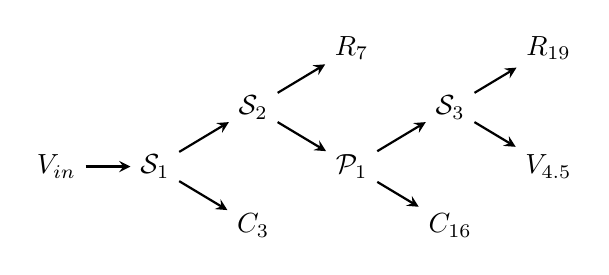
\begin{tikzpicture}[node distance=1.25cm]
            \tikzset{
                arrow/.style = {thick,->,>=stealth}
            }
            \node (Vin) {$V_{in}$};
            \node (S1)  [right of=Vin] {$\mathcal{S}_1$};
            \node (C3)  [right of=S1, below of=S1, yshift= 0.5cm] {$C_3$};
            \node (S2)  [right of=S1, above of=S1, yshift=-0.5cm] {$\mathcal{S}_2$};
            \node (R7)  [right of=S2, above of=S2, yshift=-0.5cm] {$R_7$};
            \node (P1)  [right of=S2, below of=S2, yshift= 0.5cm] {$\mathcal{P}_1$};
            \node (C16) [right of=P1, below of=P1, yshift= 0.5cm] {$C_{16}$};
            \node (S3)  [right of=P1, above of=P1, yshift=-0.5cm] {$\mathcal{S}_3$};
            \node (R19) [right of=S3, above of=S3, yshift=-0.5cm] {$R_{19}$};
            \node (V45) [right of=S3, below of=S3, yshift= 0.5cm] {$V_{4.5}$};
    
            \draw [arrow] (Vin) -- (S1);
            \draw [arrow] (S1) -- (C3);
            \draw [arrow] (S1) -- (S2);
            \draw [arrow] (S2) -- (R7);
            \draw [arrow] (S2) -- (P1);
            \draw [arrow] (P1) -- (C16);
            \draw [arrow] (P1) -- (S3);
            \draw [arrow] (S3) -- (R19);
            \draw [arrow] (S3) -- (V45);
        \end{tikzpicture}
        \caption{\label{fig:wdftree}{\it WDF tree for the Klon Centaur Feed-Forward Network 1 Circuit.
        $\mathcal{S}$ and $\mathcal{P}$ nodes refer to series and parallel adaptors respectively.}}
    \end{figure}
\end{frame}

\begin{frame}{Time-Domain Response}
    \begin{figure}
        \centering
        \includegraphics[height=2.75in]{../Paper/Figures/WDFval.png}
    \end{figure}
\end{frame}

\begin{frame}{Wave Digital Filters}
    \begin{columns}
        \begin{column}{0.5\linewidth}
            \hspace{-1ex}
            Advantages:
            \vspace{1ex}
            \begin{itemize}
                \itemsep0.5em
                \item Modularity: circuit elements and topology can be alterred on-the-fly
                \item Each element can be discretized with a different conformal map
                % \item Requires very little prior knowledge
            \end{itemize}
        \end{column}
        \begin{column}{0.5\linewidth}
            \hspace{-1ex}
            Disadvantages:
            \vspace{1ex}
            \begin{itemize}
                \itemsep0.5em
                \item Cannot model circuits with multiple nonlinearities or $\mathcal{R}$-type topologies
                \item These types of circuits can be modelled using $\mathcal{R}$-adaptors,
                but with an increase in complexity
            \end{itemize}
        \end{column}
    \end{columns}
\end{frame}

\begin{frame}{Wave Digital Filters}
    More information:
    \vspace{1ex}
    \begin{itemize}
        \itemsep0.75em
        \item Alfred Fettweis, ``Wave Digital Filters: Theory and Practice'',
        \emph{Proceedings of the IEEE}, vol. 74, no. 2, 1986
        \begin{itemize}
            \item Original reference for deriving WDF formalism
        \end{itemize}

        \item Kurt Werner, \emph{Virtual Analog Modeling of Audio Circuitry Using Wave Digital Filters},
        PhD. Thesis, Stanford University, 2016
        \begin{itemize}
            \item Great reference for deriving WDFs, including more recent advancements
            \item Expands WDFs to handle $\mathcal{R}$-type topologies and multiple nonlinearities
        \end{itemize}
    \end{itemize}
\end{frame}

\begin{frame}{Wave Digital Filters}
    More information:
    \vspace{1ex}
    \begin{itemize}
        \itemsep0.75em
        \item Fran\c{c}ois Germain, \emph{Non-oversampled physical modeling for virtual analog simulation},
        PhD. Thesis, Stanford University, 2019
        \begin{itemize}
            \item Example of independently discretizing circuit elements with Alpha Transform
        \end{itemize}

        \item Jingjie Zhang and Julius Smith, ``Real-time Wave Digital Simulation of
        Cascaded Vacuum Tube Amplifiers Using Modified Blockwise Method'',
        \emph{Proc. of the 21st International Conference on Digital Audio Effects}, 2018
        \begin{itemize}
            \item Real-time simulation of an impressively large circuit
        \end{itemize}
    \end{itemize}
\end{frame}

\begin{frame}
    \begin{centering}
        \vskip5ex plus 1filll
        {\usebeamerfont{title page title}\usebeamercolor[fg]{title page} Real-Time Neural Networks\\[1.5ex]}
        \vskip0pt plus 1filll
    \end{centering}
\end{frame}

\begin{frame}{Black Box Modelling with Neural Nets}
    Previous work: Damsk{\"a}gg et al., 2019\footcite[]{WaveNetVA}
    \vspace{1ex}
    \begin{itemize}
        \itemsep0.5em
        \item Uses a WaveNet-style, ``Temporal Convolutional Network''
        \item Used to model distortion pedal circuits
        \item Also used to model tube amp distortion\footcite[]{damskgg2018deep}
        \item Disadvantage: computationally expensive
    \end{itemize}
\end{frame}

\begin{frame}{Temporal Convolutional Networks}
    Keith Bloemer: Smart Guitar Amp\footnote{\url{https://github.com/keyth72/SmartGuitarAmp}}
    \begin{figure}
        \centering
        \includegraphics[height=2.25in]{Figures/SmartAmp.png}
    \end{figure}
\end{frame}

\begin{frame}{Temporal Convolutional Networks}
    Christian Steinmetz: Randomized Overdrive Neural Networks\footnote{\url{https://github.com/csteinmetz1/ronn}}
    \begin{figure}
        \centering
        \includegraphics[height=2.25in]{Figures/ronn-vst-ui.png}
    \end{figure}
\end{frame}

% \begin{frame}{Temporal Convolutional Networks}
%     Neural DSP (probably\dots)
%     \begin{figure}
%         \centering
%         \includegraphics[height=2.5in]{Figures/neuraldsp.png}
%     \end{figure}
% \end{frame}

\begin{frame}{Black Box Modelling with Neural Nets}
    Previous work: Parker et al., 2019\footcite[]{NLML}
    \vspace{1ex}
    \begin{itemize}
        \itemsep0.5em
        \item Uses a deep, fully-connected ``State Transition Network''
        \item Approximates a state-space solution for nonlinear distortion and filter circuits
        \item Effectively a ``grey-box'' model
    \end{itemize}
\end{frame}

\begin{frame}{State Transition Networks}
    Native Instruments: Guitar Rig 6 Pro\footnote{\url{https://blog.native-instruments.com/the-making-of-icm/}}
    \begin{figure}
        \centering
        \includegraphics[height=2.25in]{Figures/GuitarRig6.jpg}
    \end{figure}
\end{frame}

\begin{frame}{Black Box Modelling with Neural Nets}
    Previous work: Wright et al., 2019\footcite[]{VArnn}
    \vspace{1ex}
    \begin{itemize}
        \itemsep0.5em
        \item Uses a single layer recurrent neural network
        \item Used to model guitar distortion circuits
        \item Can also be used to model time-varying circuits\footcite[]{RNNtime}
    \end{itemize}
\end{frame}

\begin{frame}
    \begin{centering}
        \vskip5ex plus 1filll
        {\usebeamerfont{title page title}\usebeamercolor[fg]{title page} Real-Time Neural Networks\\[1.5ex]}
        \vskip0pt plus 1filll
    \end{centering}
\end{frame}

\begin{frame}{Black Box Modelling with Neural Nets}
    Previous work: Damsk{\"a}gg et al., 2019\footcite[]{WaveNetVA}
    \vspace{1ex}
    \begin{itemize}
        \itemsep0.5em
        \item Uses a WaveNet-style, ``Temporal Convolutional Network''
        \item Used to model distortion pedal circuits
        \item Also used to model tube amp distortion\footcite[]{damskgg2018deep}
        \item Disadvantage: computationally expensive
    \end{itemize}
\end{frame}

\begin{frame}{Temporal Convolutional Networks}
    Keith Bloemer: Smart Guitar Amp\footnote{\url{https://github.com/keyth72/SmartGuitarAmp}}
    \begin{figure}
        \centering
        \includegraphics[height=2.25in]{Figures/SmartAmp.png}
    \end{figure}
\end{frame}

\begin{frame}{Temporal Convolutional Networks}
    Christian Steinmetz: Randomized Overdrive Neural Networks\footnote{\url{https://github.com/csteinmetz1/ronn}}
    \begin{figure}
        \centering
        \includegraphics[height=2.25in]{Figures/ronn-vst-ui.png}
    \end{figure}
\end{frame}

% \begin{frame}{Temporal Convolutional Networks}
%     Neural DSP (probably\dots)
%     \begin{figure}
%         \centering
%         \includegraphics[height=2.5in]{Figures/neuraldsp.png}
%     \end{figure}
% \end{frame}

\begin{frame}{Black Box Modelling with Neural Nets}
    Previous work: Parker et al., 2019\footcite[]{NLML}
    \vspace{1ex}
    \begin{itemize}
        \itemsep0.5em
        \item Uses a deep, fully-connected ``State Transition Network''
        \item Approximates a state-space solution for nonlinear distortion and filter circuits
        \item Effectively a ``grey-box'' model
    \end{itemize}
\end{frame}

\begin{frame}{State Transition Networks}
    Native Instruments: Guitar Rig 6 Pro\footnote{\url{https://blog.native-instruments.com/the-making-of-icm/}}
    \begin{figure}
        \centering
        \includegraphics[height=2.25in]{Figures/GuitarRig6.jpg}
    \end{figure}
\end{frame}

\begin{frame}{Black Box Modelling with Neural Nets}
    Previous work: Wright et al., 2019\footcite[]{VArnn}
    \vspace{1ex}
    \begin{itemize}
        \itemsep0.5em
        \item Uses a single layer recurrent neural network
        \item Used to model guitar distortion circuits
        \item Can also be used to model time-varying circuits\footcite[]{RNNtime}
    \end{itemize}
\end{frame}

\begin{frame}
    \begin{centering}
        \vskip5ex plus 1filll
        {\usebeamerfont{title page title}\usebeamercolor[fg]{title page} Real-Time Neural Networks\\[1.5ex]}
        \vskip0pt plus 1filll
    \end{centering}
\end{frame}

\input{Slides/Neural/Previous.tex}
\input{Slides/Neural/RNN.tex}
\input{Slides/Neural/Training.tex}
\input{Slides/Neural/Summary.tex}

\begin{frame}{Recurrent Neural Network: Training}
    Training: 500 epochs, $\sim 8$ hours
    \begin{figure}
        \centering
        \includegraphics[height=2.5in]{../Paper/Figures/Training.png}
    \end{figure}
\end{frame}

\begin{frame}{Recurrent Neural Network: Training}
    Training results (time domain)
    \begin{figure}
        \centering
        \includegraphics[height=2.5in]{../Paper/Figures/TimeDomain.png}
    \end{figure}
\end{frame}

\begin{frame}{Recurrent Neural Network: Training}
    Training results (frequency domain)
    \begin{figure}
        \centering
        \includegraphics[height=2.5in]{../Paper/Figures/FreqDomain.png}
    \end{figure}
\end{frame}

\begin{frame}{Recurrent Neural Networks}
    \begin{columns}
        \begin{column}{0.5\linewidth}
            \hspace{-1ex}
            Advantages:
            \vspace{1ex}
            \begin{itemize}
                \itemsep0.5em
                \item Efficient black-box modelling technique for distortion circuits
                \item Can potentially include control parameters
            \end{itemize}
        \end{column}
        \begin{column}{0.5\linewidth}
            \hspace{-1ex}
            Disadvantages:
            \vspace{1ex}
            \begin{itemize}
                \itemsep0.5em
                \item Large networks can be computationally expensive
                \item Must be used at the same sample rate as training data
                \item Can be difficult to train with control parameters
            \end{itemize}
        \end{column}
    \end{columns}
\end{frame}

\begin{frame}{Neural Networks: Future Work}
    Computational Efficiency
    \begin{itemize}
        \itemsep0.5em
        \item Dense, recurrent, and convolutional layers often require nonlinear activation functions, like $\tanh$
        \item In DSP, we often use fast approximations, or look-up tables
        \item Can we use function approximations in neural networks?
        \begin{itemize}
            \itemsep0em
            \item Is it better to train with approximations, or train with full precision, and use approximations for real-time implementation?
            \item Similar to questions in TinyML about weight quantization
        \end{itemize}
    \end{itemize}
\end{frame}

\begin{frame}{Neural Networks: Future Work}
    Sample Rate
    \begin{itemize}
        \itemsep0.5em
        \item Currently most networks must be used at the same sample rate as the training data
        \item Can one network to be used for a range of sample rates?
        \begin{itemize}
            \itemsep0em
            \item Sample rate as input?
            \item Transform network weights?
            \item Fractional delay (RNN only)?
        \end{itemize}
        \item What about aliasing?
    \end{itemize}
\end{frame}


\begin{frame}{Recurrent Neural Network: Training}
    Training: 500 epochs, $\sim 8$ hours
    \begin{figure}
        \centering
        \includegraphics[height=2.5in]{../Paper/Figures/Training.png}
    \end{figure}
\end{frame}

\begin{frame}{Recurrent Neural Network: Training}
    Training results (time domain)
    \begin{figure}
        \centering
        \includegraphics[height=2.5in]{../Paper/Figures/TimeDomain.png}
    \end{figure}
\end{frame}

\begin{frame}{Recurrent Neural Network: Training}
    Training results (frequency domain)
    \begin{figure}
        \centering
        \includegraphics[height=2.5in]{../Paper/Figures/FreqDomain.png}
    \end{figure}
\end{frame}

\begin{frame}{Recurrent Neural Networks}
    \begin{columns}
        \begin{column}{0.5\linewidth}
            \hspace{-1ex}
            Advantages:
            \vspace{1ex}
            \begin{itemize}
                \itemsep0.5em
                \item Efficient black-box modelling technique for distortion circuits
                \item Can potentially include control parameters
            \end{itemize}
        \end{column}
        \begin{column}{0.5\linewidth}
            \hspace{-1ex}
            Disadvantages:
            \vspace{1ex}
            \begin{itemize}
                \itemsep0.5em
                \item Large networks can be computationally expensive
                \item Must be used at the same sample rate as training data
                \item Can be difficult to train with control parameters
            \end{itemize}
        \end{column}
    \end{columns}
\end{frame}

\begin{frame}{Neural Networks: Future Work}
    Computational Efficiency
    \begin{itemize}
        \itemsep0.5em
        \item Dense, recurrent, and convolutional layers often require nonlinear activation functions, like $\tanh$
        \item In DSP, we often use fast approximations, or look-up tables
        \item Can we use function approximations in neural networks?
        \begin{itemize}
            \itemsep0em
            \item Is it better to train with approximations, or train with full precision, and use approximations for real-time implementation?
            \item Similar to questions in TinyML about weight quantization
        \end{itemize}
    \end{itemize}
\end{frame}

\begin{frame}{Neural Networks: Future Work}
    Sample Rate
    \begin{itemize}
        \itemsep0.5em
        \item Currently most networks must be used at the same sample rate as the training data
        \item Can one network to be used for a range of sample rates?
        \begin{itemize}
            \itemsep0em
            \item Sample rate as input?
            \item Transform network weights?
            \item Fractional delay (RNN only)?
        \end{itemize}
        \item What about aliasing?
    \end{itemize}
\end{frame}


\begin{frame}
    \begin{centering}
        \vskip5ex plus 1filll
        {\usebeamerfont{title page title}\usebeamercolor[fg]{title page} Real-Time Implementation\\[1.5ex]}
        \vskip0pt plus 1filll
    \end{centering}
\end{frame}

\begin{frame}{Klon Centaur Circuit Schematic}
    \begin{figure}
        \centering
        \includegraphics[width=5.75in]{../Paper/Figures/FullCircuit.png}
    \end{figure}
\end{frame}

\begin{frame}{Implementation}
    \begin{columns}
        \begin{column}{0.45\linewidth}
            Non-ML Implementation
            \begin{itemize}
                \item Use a combination nodal analysis, WDFs
                \item Control parameters for Treble, Gain, Level
            \end{itemize}
        \end{column}
        \begin{column}{0.55\linewidth}
            ML Implementation
            \begin{itemize}
                \item RNN model for Gain Stage, nodal analysis elsewhere
                \item Fade between models for variable Gain control
                \item Custom GRU and Dense layer implementations in C++
            \end{itemize}
        \end{column}
    \end{columns}
\end{frame}

\begin{frame}{RNN Inferencing Engine}
    Tensorflow Lite
    \begin{itemize}
        \item Converts a Tensorflow model to a format that can be run on embedded devices
        \item Support for GRUs is still experimental
        \item Real-time audio concerns: no thread locks, no memory allocation on real-time audio thread
    \end{itemize}
\end{frame}

\begin{frame}{RNN Inferencing Engine}
    Custom engine: Eigen
    \begin{itemize}
        \item Eigen is a linear algebra C++ library with SIMD support for matrix/vector operations
        \item Custom implementations of GRU and fully connected layers, validated against Tensorflow
        \item Can be difficult to compile on embedded devices
    \end{itemize}
\end{frame}

\begin{frame}{RNN Inferencing Engine}
    Custom engine: C++ STL
    \begin{itemize}
        \item Optimized algorithms for operations such as \lstinline{std::inner_product}
        \item Custom implementations of GRU and fully connected layers, validated against Tensorflow
        \item Can be compiled on most embedded devices
    \end{itemize}
\end{frame}

\begin{frame}{Implementation}
    Desktop Audio Plugin (JUCE/C++)
    \begin{figure}
        \centering
        \includegraphics[height=2.5in]{../Paper/Figures/Plugin.png}
    \end{figure}
\end{frame}

\begin{frame}{Implementation}
    Teensy 4.0, Teensy Audio Shield, Teensy Audio Library
    \begin{figure}
        \centering
        \includegraphics[height=2.5in]{../Paper/Figures/Teensy.jpg}
    \end{figure}
\end{frame}

\begin{frame}{Results: Performance}
    Compute time per second of audio.
    \begin{table}[h!]
        \centering
         \begin{tabular}{||c | c | c||} 
         \hline
         Block Size & NonML Speed & ML Speed \\
         \hline\hline
         8    & 0.0723437 & 0.0528792 \\
         16   & 0.0703079 & 0.0510437 \\
         32   & 0.0652856 & 0.0511147 \\
         64   & 0.0662835 & 0.0502434 \\
         128  & 0.0666593 & 0.0495194 \\
         256  & 0.0696844 & 0.0480298 \\
         512  & 0.0669037 & 0.0477946 \\
         1024 & 0.060816  & 0.0488841 \\
         2048 & 0.0695175 & 0.0488309 \\
         4096 & 0.0623839 & 0.0472191 \\
         \hline
         \end{tabular}
    \end{table}
\end{frame}

\begin{frame}{Results: Summary}
    \begin{itemize}
        \item Subjectively, non-ML and ML models sound very similar.
        \item ML model has slightly damped high frequency response,
            (not a big deal on guitar input; more noticeable on other audio).
        \item ML model is more efficient!
    \end{itemize}
\end{frame}

\begin{frame}{Takeaways}
    \begin{itemize}
        \itemsep0.75em
        \item 3 methods for modelling circuits:
        \begin{itemize}
            \item Nodal Analysis (simplest)
            \item Wave Digital Filters (modular)
            \item Neural Networks (experimental)
        \end{itemize}
        \item Modelling circuits with neural networks can be done, but more research/experimentation is needed
        \item Desktop vs. Embedded:
        \begin{itemize}
            \item Memory management
            \item Processing power (floating point processing, SIMD)
            \item Price
        \end{itemize}
    \end{itemize}
\end{frame}


\begin{frame}{Links}
    \begin{itemize}
        \itemsep0.75em
        \item \href{https://arxiv.org/abs/2009.02833}{Technical Paper}
        \item \href{https://github.com/jatinchowdhury18/KlonCentaur}{Source Code (and plugin download)}
        \item \href{https://www.youtube.com/playlist?list=PLrcXtWXbPsj11cNBamVyMmDcWY1SXZHvz}{Video Demos}
    \end{itemize}
\end{frame}

\begin{frame}{Acknowledgements}
    \begin{itemize}
        \item Pete Warden and the EE 292D class, for insipiring this project
        \item Julius Smith, Kurt Werner, and Jingjie Zhang, for assistance with WDFs
    \end{itemize}
\end{frame}

\begin{frame}
    \begin{centering}
        \vskip5ex plus 1filll
        {\usebeamerfont{title page title}\usebeamercolor[fg]{title page} Thank You!\\[1.5ex]}
        \vskip0pt plus 1filll
    \end{centering}
\end{frame}

\fullslideimg{Figures/end.jpg}

\end{document}
